\documentclass[12pt,a4]{report}
\usepackage[frenchb]{babel}

\usepackage[usenames,dvipsnames]{color}
\usepackage[utf8]{inputenc}
\usepackage{textcomp}
\usepackage[T1]{fontenc}
\usepackage{lmodern}	
\usepackage{bibunits}
\usepackage{graphicx}
\usepackage{wrapfig}
\usepackage{glossaries}
\makeglossaries
\usepackage{float}
\usepackage{cite}
\usepackage{caption}
\usepackage{amsmath,mathtools}
\usepackage{subcaption}

\newacronym{w3c}{W3C}{World Wide Web Consortium}
\newacronym{rdf}{RDF}{Resource Description Framework}
\newacronym{trdf}{tRDF}{Temporal RDF}
\newacronym{strdf}{stRDF}{spatial and temporal Resource Description Framework}
\newacronym{lod}{LOD}{Linked Open Data, Web de données}
\newacronym{sparql}{SPARQL}{Protocol and RDF Query Language}
\newacronym{owl}{OWL}{Web Ontology Language}
\newacronym{stsparql}{stSPARQL}{spatial and temporal Protocol and RDF Query Language}
\newacronym{uri}{URI}{Uniform Resource Identifier}
\newacronym{iri}{IRI}{Internationalized Resource Identifier }
\newacronym{sql}{SQL}{Structured Query Language}
\begin{document}
\chapter{État de l'art}
\section{Introduction}
\paragraph{}
Les bases de connaissances jouent un rôle de plus en plus important dans l'intelligence du Web et dans la recherche. Ainsi elles favorisent l'intégration de l'information. La plupart des bases de connaissances contiennent des informations relatives à des actions dans le temps qui ne possèdent pas la bonne structure capable de relier directement l'événement au temps ou à la période associer à cette événement.
Ces bases de connaissance ne portent que sur des domaines spécifiques (les entreprises, les films, la musique, les livres, les plublications scientifiques etc..), sont créées par des ingénieurs de connaissance. Dans ce contexte, on cite Wikipédia qui est devenue l'une des sources de connaissances centrale de l'humanité. Cette encyclopédie libre est entretenue par des milliers de contributeurs.
\subparagraph{}
Notre étude s'appuie sur DBpedia une source gigantesque de connaissances par l'extraction des informations structurées à partir de Wikipédia pour rendre ces informations utiles et également accessibles sur le Web. La base de connaissance DBpedia à plusieurs avantages sur les bases de connaissances existante : elle couvre plusieurs domaines, elle évolue automatiquement avec les changements de Wikipédia, elle est multilingue et accessible sur le Web. 
Comme DBpedia couvre un large éventail de domaines et contient environ 4,8 milliards de triplets RDF qui couvrent des domaines divers, un nombre croissant d'éditeurs de données ont commencé à mettre des liens RDF à partir de leurs sources de données à DBpedia.
\subparagraph{}
Durant cette étude, nous avons travaillé sur les bases de connaissances pour annoter temporellement leurs contenus. Nous avons choisi praticulièrement DBpedia et nous avons développé un système automatique d'extraction d'informations qui convertit une partie du contenu de DBpedia dans une riche et plus structuré base de données temporelle que nous avons appelé SPOTbase.
\subparagraph{}
SPOTbase est une base de connaissance, regroupe des triplets annotés générer automatiquement à l'aide d'une procédure de ``mapping`` que nous avons implémenté à partir de DBpedia.
Nous avons réussi à former envirant 300 quadruplets et beaucoup plus dans certains cas pour un seul couple qui valide bien notre hypothèse.
\subparagraph{}
Dans ce chapitre, nous introduisons les différentes, modèles, paradigmes et technologies que nous allons utiliser dans notre étude ainsi que les travaux de recherche liés à cette problématique ; tout en essayant d'analyser les différentes approches. Ceci est dans le but de mettre en place la solution que nous avons proposée.
\section{Positionnement}
\paragraph{}
Notre étude a la particularité d’englober le domaine de la fouille de données et du Web sémantique. 
En effet, nous utilisons les techniques de la fouille pour l'extraction des données depuis les différentes sources d'informations; et le Web sémantique afin de donner aux métadonnées une nouvelle structure plus lisible par la machine. Notre travail vise à enrechir la sémantique des triplets RDF dans les bases de connaissances avec des annotations temporelles permettant de donner aux triplets une sémantique valide dans le temps.
\subparagraph{}
Dans cette section on présente les technologies du Web sémantique que nous avons utilisées, puis nous effectuerons une étude autour des travaux de recherche qui précèdent notre étude tout en introduisant les concepts à développer et la problématique de notre sujet.
\section{Technologies du Web sémantique}
\subsection{Intérêt du Web sémantique}
\paragraph{}
Le Web sémantique est un domaine de recherche né des travaux de Tim Berners-Lee~\cite{Berners-lee2001}. Ses efforts avaient pour but d'ajouter du sens aux contenus du Web et d'automatiser l'accès à l'information utile sur le Web. La question n’est pas d'ajouter une autre alternative au Web. Il s’agit plustôt d'étendre le Web actuel dans le but d'utiliser et de manipuler le maximum de son contenu informatiquement dont l’objectif est de permettre à des programmes informatiques de traiter un ensemble étendu de données issues du Web.
\subsection{Modèle RDF}
\paragraph{}
Au centre du Web sémantique, comme la brique d’argile qui permet d’ériger les plus grands édifices, se trouve le modèle \gls{rdf}. RDF\footnote{http://www.w3.org/RDF/} est un standard de \gls{w3c}, il se base sur un modèle de graphe sous forme de triplets (sujet, prédicat, objet) qui permettent d'exprimer tout les type d'assertions. Il s’agit d’un cadre de description de ressources, d’une façon formelle sur le Web.
C’est la première brique de standard du Web sémantique qui recouvre à la fois un modèle et plusieurs syntaxes pour publier des données variées sur le Web.
\subparagraph{}
Dans RDF :
\newline
\begin{itemize}
\item Les ressources sont un concept de base du Web sémantique. Tout ce qui peut être référencé est une ressource. Dans un contexte plus technique, on déduit que tout ce qui peut être identifié par un \gls{uri} / \gls{iri} peut être considéré comme une ressource.
\item Un ensemble d’attributs décrivent la ressource, qui possède des caractéristiques et des relations avec d’autres ressources.
\item Le cadre standardise la syntaxe de ces descriptions, mais aussi les modèles et les langages.
\end{itemize}
\subparagraph{}
Rapellons que la plus petite structure de description en RDF est le triplet.
\begin{figure}[H]
\centering
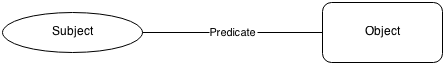
\includegraphics[width=8cm]{tripletrdf.png}
\caption{triplet RDF}
\end{figure}
\subparagraph{}
Un triplet décrit une ressource, l’associe à une propriété et à une valeur de cette propriété qui peut être une nouvelle ressource liée. 
\newline
Par exemple, “Moncef a écrit une page QuadsRDF.html à propos des quadruplets RDF” peut être décomposée en deux triplets ayant comme sujet “QuadsRDF.html”: <QuadsRDF.html, auteur, Moncef> et <QuadsRDF.html, thème, quadruplets RDF>.
\newline
Par conséquent, les suivants <Sujet,Prédicat,Objet>, c'est-à-dire les suivants triplets RDF peuvent être exprimés :
\begin{description}
\item[\ \ \textbullet]  <http://www.w3.org/TR/2014/REC-n-quads/>, <http://www.w3.org/
2014/N-QuadsReports/index.html\#author>, ``Moncef``.
\item[\ \ \textbullet]  <http://www.w3.org/TR/2014/REC-n-quads/>, <http://www.w3.org/
2014/N-QuadsReports/index.html\#topic>, <http://www.w3.org/2014/
N-Quads\#RDFquad>
\end{description}
On peut schématiser cela de la manière suivante :
\begin{figure}[H]
\centering
\centering
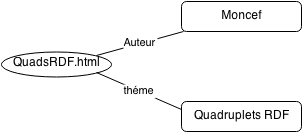
\includegraphics[width=8cm]{Diag.png}
\caption{Deux triplets liés au même sujet}
\end{figure}
\newpage
\subsection{SPARQL}
\paragraph{}
Si RDF fournit un modèle universel de représentation de métadonnées, d'autres niveaux de traitements ont été standardisés au-dessus de lui et notamment l'interrogation de ces métadonnées. 
\gls{sparql} fournit le langage d'interrogation du Web sémantique, et en cela il est à RDF ce que \gls{sql} est aux bases de données relationnelles.
\subparagraph{}
SPARQL est un langage d'interrogation de graphes RDF dont l'énoncé de base est lui aussi un triplet (ressource, propriété, valeur) il est une recommandation du W3C depuis juillet 2008.
Poser une question en SPARQL consiste à écrire un graphe requête pour lequel on cherche des occurences dans le graphe cible.
\subsection{N-Quads}
\paragraph{}
N-Quads\footnote{http://sw.deri.org/2008/07/n-quads/}, un format qui s'étend N-Triples\footnote{http://www.w3.org/2001/sw/RDFCore/ntriples/} (une simple syntaxe de ligne délimitée ``line-delimited`` pour les graphes RDF) avec le contexte. Chaque triplet dans un document N-Quads peut avoir une valeur de contexte en option :
<subjet> <prédicat> <objet> <contexte>.
\subparagraph{}
La notion de provenance est essentielle lors de l'intégration des données provenant de différentes sources ou du Web. Le contexte indique généralement la provenance d'une déclaration donnée.
\subsection{Ontologies}
\paragraph{}
La définition de référence d’une ontologie provient de Gruber~\cite{gruber1995}  :  {\it `` Une ontologie est la spécification d’une conceptualisation. [...] Une conceptualisation est une vue abstraite et simplifiée du monde que l’on veut représenter.``} Le terme vocabulaire est aussi utilisé en tant que synonyme d’ontologie.
\subparagraph{}
\textbf{Exemple de vocabulaire RDF} On considère les relations suivantes : \textit{dc:title}, \textit{dc:author} et \textit{foaf:knows}. Celles-ci ont été définies dans les vocabulaires Dublin Core et FOAF. Un vocabulaire modélise un domaine particulier : concepts, relations. Par exemple FOAF modélise les personnes et leurs relations entre elles. Il identifie les classes Person, Agent, Organisation, etc... et les relations \textit{firstName}, \textit{familyName}, \textit{knows}, \textit{birthday}, etc... Le vocabulaire structure ensuite ces  éléments : \textit{Person} est une sous-classe de \textit{Agent}, \textit{familyName} a pour domaine la classe \textit{Person}, etc...
\subparagraph{}
\textbf{RDF Schema, ou RDFS}, est le langage de description de vocabulaire historiquement associé à RDF. Il s'agit en effet du premier des langages de description de vocabulaire développés pour le Web de données. RDFS permet de spécifier des ontologies dites légères, c'est-à-dire de nommer des classes et des propriétés, de donner la signature de ces propriétés et de définir une organisation hiérarchique de ces classes et propriétés.
\subparagraph{}
\textbf{\gls{owl}}, est un langage de définition d'ontologie pour le Web sémantique. Il est beaucoup plus expressif que RDF Schema. OWL permet d'exprimer les notions d'équivalence de classes ou de propriétés, d'égalité de ressources, de différence, de contrainte... OWL 1 est une recommandation du W3C depuis 2004.
\newpage
\subsection{Bases de Connaissances}
\paragraph{}
Une base de connaissances regroupe des informations spécifiques à un domaine donné, sous un format exploitable par un ordinateur. Elle peut contenir des régles, des faits ou d'autres représentations. Les bases de connaissances regroupent des informations structurées. C’est dans ce contexte que nous cherchons à exploiter ces informations pour les mettre dans une nouvelle structure plus facilement exploitable par la machine. 

\subsubsection{DBpedia}
\paragraph{}

C'est un projet universitaire et communautaire d’extraction et d’exploitation automatiques des données à partir de wikipedia. C’est également un ensemble de données structurées et normalisées au format du Web sémantique.
\begin{wrapfigure}{r}{0.7\textwidth}
\vspace{-10pt}
\begin{center}
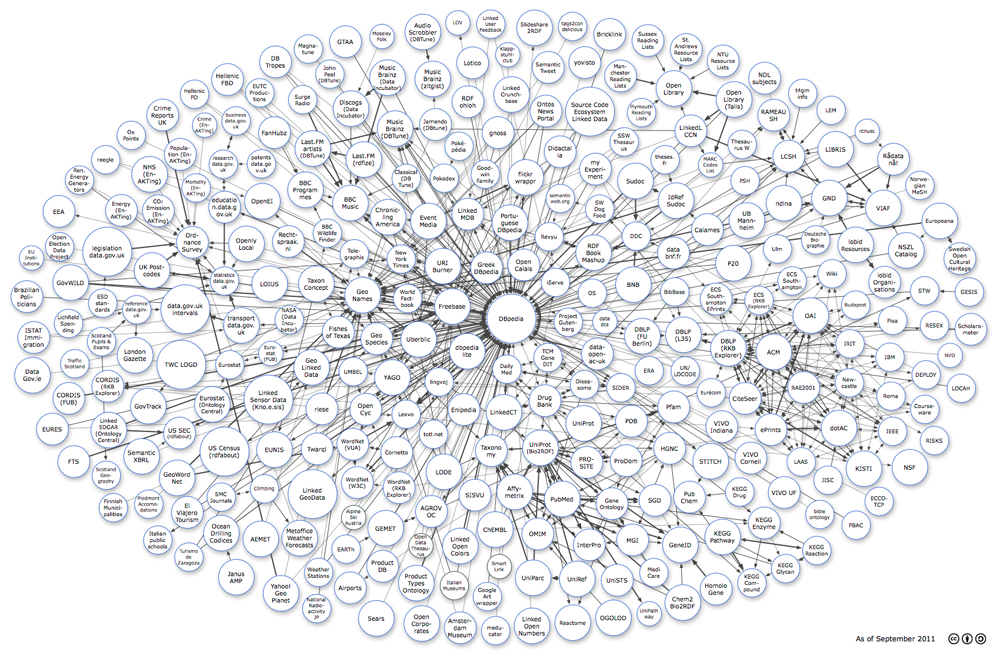
\includegraphics[width=0.50\textwidth]{dbpedia.png}
\end{center}
\vspace{-15pt}
\caption{DBpedia}
\vspace{-10pt}
\end{wrapfigure}
DBpedia 3.9 est la dernière version de DBpedia datant de Juin 2013.
\subparagraph{}
Cette base de connaissances est écrite en Scala et Java. Elle adopte les normes du Web sémantique et du réseau Linked Open Data. Pour chaque document encyclopédique, il existe une page de ressources contenant toutes les données et leur description sous forme de triplets RDF. Ces triplets peuvent représenter une information telle que Obama est le président des État-Unis, ($Obama$, $PresidentOf$, $US$).
DBpedia est conçu par ces auteurs comme l'un des noyaux du Web émergent sous le nom de Web de données. Les triplets dans cette base de connaissance représentent des faits du monde réel qui doivent avoir une sémantique correcte et valide.

\newpage
\subsubsection{YAGO}
YAGO\footnote{http://www.mpi-inf.mpg.de/yago-naga/yago/} est une large base de connaissances sémantiques, délivrée de Wikipedia, WordNet et GeoNames. Actuellement elle contient plus de 10 millions d’entités (personnes, organisations, villes, etc...) et plus de 120 millions de faits au sujet de ces entités.
\newline
Les caractéristiques principales de YAGO :
\begin{itemize}
\item YAGO combine la taxonomie propre de WordNet\footnote{http://fr.wikipedia.org/wiki/WordNet} avec la richesse du système de catégorie Wikipedia, l'attribution des entités à plus de 350000 catégories.
\item YAGO est une ontologie qui attache une dimension temporelle et spatiale à plusieurs de ces faits et entités.
\end{itemize}
\begin{figure}[H]
\centering
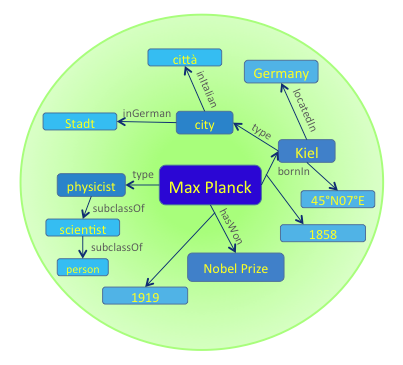
\includegraphics[width=10cm]{yago.png}
\caption{YAGO}
\end{figure}
\subsubsection{Wikidata}
\paragraph{}
C'est un projet d'une base de données éditée d'une manière collaborative cela pour aider à la mise à jour des données de Wikipédia. Ce projet est lancé par Wikimedia Deutschland. Wikidata est déstiné à fournir une source commune de données objectives, telles que les dates de naissances ou bien le PIB des pays, qui pourront être utilisées dans tous les articles des différentes versions linguistiques de wikipédia, une mise à jour de wikidata  pouvant être alors répercutée automatiquement sur l'ensemble des wikipédias en différentes langues.   
\begin{figure}[H]
\centering
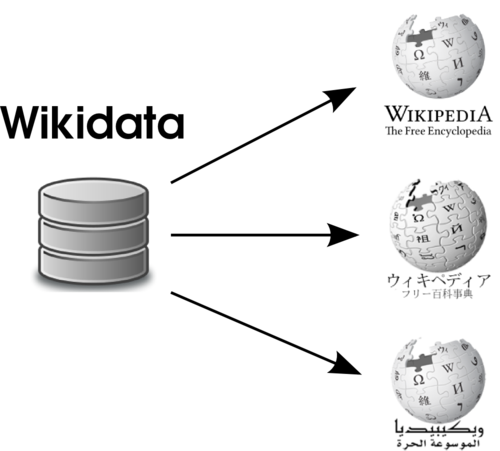
\includegraphics[width=12cm]{wikidatawikipedia.png}
\caption{Wikidata}
\end{figure}

\section{Différentes approches d'annotation temporelle}			
\paragraph{}
Dans le domaine du Web sémantique, il y a plusieurs extensions de RDF qui ont été proposées pour : la vérité, la confiance, la certitude et le temps.
Par exemple : pour la verité de certains triplets où le degré de vérité est entre $0$ et $1$, l’instance “Rome est une grande ville de degré 0.8” peut être représentée par $(Rome, type,grande{\_}ville) : 0.8$.
\subparagraph{}
De même pour la certitude, une autre forme a été proposé :
$(Max,hasSupervisor : (0.9,2003),William)$ à la forme générale suivante $(s, p : (x,t),o)$
\newline
Dans ce dernier exemple on remarque que l'annotation est sous forme de couple$(x, t)$ où $x$ la certitude est représentée sous forme d'un pourcentage 90\% et $t$ le temps sous forme d'une année $2003$.
\subsection{L'annotation temporelle}
\paragraph{}
La nécessité de l’annotation temporelle sur les documents Web a été évoquée dans des nombreux travaux de recherche. La première approche formelle au problème de modélisation et d’interrogation temporelle en RDF a été introduite par Gutierrez et al~\cite{gutierrez2005}.
\subparagraph{}
Ensuite, Udrea et al~\cite{udrea2006} ont travaillé sur la notion d'annoter temporellement les graphes RDF et depuis plusieurs travaux de recherche ont évoqué cette problématique.
Ces derniers définissent que le triplet annoté de la forme suivante $(s,p:t,o)$ où $t$ est une étiquette temporelle. De plus ils ont donné des algorithmes pour interroger les données RDF annotées.
\subparagraph{}	
Plusieurs études de recherche ont défini des modèles de représentation du temps dans les graphes RDF. Nous avons cherché à étudier ces différentes représentations qui n'ont malheureusement pas donné un lien à aucune implémentation concrète. Par la suite, nous présenterons notre approche et une implémentation du modèle que nous avons proposé.  
\subsection{RDF Temporel ou tRDF}
\paragraph{}
Pour introduire \gls{trdf}, on commence par les exemples suivants:
\newline
Il y a des triplets comme par exemple : ``Mary est toujours la mère de John`` qui n'ont pas une caractéristique temporelle explicite parce qu’ils sont toujours valide. Mais il y a aussi des triplets ayant une valeur vrai que dans une plage temporelle bien précise, par exemple : ``Bill Clinton est le président de Etats-Unis``, n'est valide que dans l'intervalle $[1993-2001]$.
\subparagraph{}
Donc il y a des triplets qui ne peuvent être reconnus que dans des périodes temporelles précises.
\paragraph{}
D'après Andrea et al~\cite{pugliese2008} l’annotation tRDF peut être exprimée de la manière suivante ($n$ est un nombre entier, $T$ appartient à un intervalle de temps, $s$ le sujet, $p$ le prédicat, $v$ l'objet) :
\begin{enumerate}
\item ($s$, $p$ : {$T$}, $v$), ce type de triplet représente une relation entre le sujet et le prédicat et l'objet dure un temps $T$ (dans n'importe quel point de temps dans $T$).
\item ($s$, $p$ : <$n$ : $T$>, $v$), ce triplet présente une relation entre $s$, $p$ et $v$ qui dure au moins $n$ point de temps différents dans $T$.
\item ($s$, $p$ : [$n$ : $T$], $v$), ce triplet présente une relation entre $s$, $p$ et $v$ qui dure au plus $n$ points de temps différents dans $T$.
\end{enumerate}
\subparagraph{}
Divers représentation de l'annotation temporelle des triplets RDF ont été proposées. Nous avons remarqué des fois une similarité entre eux ainsi : ($s$, $p$ : {$T$}, $v$) et ($s$, $p$, $v$): $T$ qui sont équivalent sémantiquement.	
\subsection{L'importance de l'annotation temporelle dans le Web de données}
\subsubsection{Présentation du LOD}
\paragraph{}
\gls{lod}\footnote{http://linkeddata.org/}, est un moyen de publier des données structurées sur le Web où les données contenues dans des bases de données sont exposées avec leur sémantique, ce qui donne la possibilité aux métadonnées d'être connectées et enrichies d'une manière solide, et permet également d'avoir plusieurs représentations d'un même contenu et de faire des rapprochements entre des ressources connexes.
\subparagraph{}
Au cours des dernières années, le Web de données a développé dans une grande fusion, de divers ensembles de données provenant de plusieurs domaines. Ce dernier décrit les ressources identifiées par des \gls{uri} en représentant leurs propriétés et des liens vers d’autres ressources. L'ensemble des données fournit des connaissances du monde réel.
\subsubsection{Relation entre l'annotation temporelle et LOD}
\paragraph{}
Les informations sur un intervalle temporel de validité pour les évènements décrits par des triplets RDF, jouent un rôle important dans plusieurs d'applications.
Un grand nombre de triplets dans LOD ne sont valides que dans un certain intervalle de temps qu'ils appellent la portée de leurs temps.
Par exemple dans DBpedia ils indiquent que ``Mario Balotelli joue pour les équipes AC Lumezzane et le Milan AC``. Lorsqu'on modélise des connaissances du monde réel, Mario Balotelli ne peut pas jouer en même temps avec AC Lumezzane et le Milan AC.
\subparagraph{}
Les logiques temporelles d'informations ont besoin d'avoir de la protée temporelle des faits tels que ``Mario Balotelli joue pour l'équipe AC Milan``.
Une approche a été proposée pour détecter la portée des évènements visés par des triplets RDF par Rule et al~\cite{rula2014} est composé de quatre étapes principales~:
\begin{itemize}
\item Les données du document Web sont normalisées pour tenir compte de l’importance des dates figurants dans les documents.
\item La sortie de la phrase est comparée avec un ensemble d’intervalles de temps pertinents pour obtenir des notes de significations pour chaque intervalle.
\item Un ensemble d’intervalles plus importants est sélectionné.
\item Les intervalles sélectionnés sont fusionnés lorsque c’est possible.
\end{itemize}
\subparagraph{}
La plateforme DeFacto (Deep Fact Validation)~\cite{lehmann2012} a été utilisée pour la validation des états en cherchant des sources qu'elle confirme sur le Web.
\subparagraph{}
Les triplets sont représentés par des faits et peuvent être associés à un contexte temporel.
Par exemple, $<Balotelli, team, AC Milan>$ se réfère à un événement de [$2003-2009$], une annotation temporelle est rattachée au fait comme suit $<f, [ti,tj]>$.
\subparagraph{}
Cette approche combine deux types d'informations~: les informations temporelles recueillies dans des documents Web et les informations temporelles contenues dans les bases de connaissances, pour associer des intervalles de temps aux triplets RDF.
\subsection{Temps valide des triplets dans les données géospatiales liées}
\paragraph{}
Bereta et al~\cite{bereta2013} introduisent la composante temporelle des données du modèle stRDF et le langage de requêtes stSPARQL, récemment proposés pour la présentation et l’interrogation des données géospatiales liées qui changent dans le temps.
\subparagraph{}
L’introduction du temps dans les modèles de données et les langages de requêtes a été l’objet de recherches approfondies dans le champs des bases de données relationnelles.
\newline
Les trois types distincts de temps qui ont été étudiées~:
\begin{itemize}
\item L'action temporelle indépendante, par exemple ($01/12/1954$ c’est l’anniversaire de John).
\item Le temps d’évènement ou un fait vrai dans l’application ( John a été professeur entre [$2001-2012$]).
\item Le délais de transaction est le moment où un fait est en cours dans la base de données (l’heure système $h$ présente l’heure exact quand John est un professeur [$2001-2012$]).
\end{itemize}
\paragraph{}
Bereta et al~\cite{bereta2013} présentent également le concept de horodatages anonymes dans les graphes RDF, par exemple le quadruplet(quad) de la forme $(s, p, o)[t]$, où $t$ est une horloge ou un timestamp $x$ anonyme déclarant que le triplet est valable dans un certain point de temps inconnu.
\subparagraph{}
L’idée principale est d’intégrer les informations géospatiales pour le modèle de graphe RDF temporel. Le langage d’interrogation \gls{stsparql}\footnote{http://www.strabon.di.uoa.gr/stSPARQL}, ajoute deux nouveaux types de variables spatiales et temporelles, aux variables SPARQL standards.
\subsection{Base de données temporelles}
\paragraph{}
Une base de données temporelle est une base de données avec des aspects de temps intégrés (temps-valide, temps-transaction), c'est-à-dire un modèle de données temporelles et une version temporelle du langage structuré de requête (SPARQL, SQL).
\subparagraph{}
En effet, le \textit{temps valide} dénote la période de temps durant laquelle un fait est vrai par rapport à la réalité.
Le \textit{temps-transaction} est la période de temps pendant laquelle un fait est stocké dans une base de données.
\paragraph{}
Dans le contexte de l'annotation temporelle des graphes RDF, les besoins se résument comme suit~:
\begin{itemize}
\item L'accès à des différentes versions d’une ontologie.
\item Récupération des informations passées sur les sites Web.
\item La distribution des mises à jour des journaux.
\end{itemize}
\subparagraph{}
Antoniou et al~\cite{antoniou2004} présentent une ontologie du service Web, pour monter qu'une ontologie peut passer par plusieurs états dont l'objectif est d'analyser et de justifier les besoins cités auparavant.
\paragraph{}
Une base de données temporelle peut être exprimée comme un répertoire d'informations temporelles.
Gutiérrez et al~\cite{gutierrez2007} montrent qu'il y aura deux manières pour ajouter des dimensions temporelles dans un graphe RDF intemporel~:
\begin{itemize}
\item Étiqueter les éléments soumis à des changements pour les triplets par exemple à chaque changement un nouveau graphe sera créé et l’ancien état sera stocké quelque part.
\item Versionner, c'est le capture de temps de transaction. D'après Gutiérrez et al~\cite{gutierrez2007} l’étiquetage est mieux que les versions pour les raisons suivantes:
\begin{itemize}
\item Il conserve le principe de la nature distribuée et extensible de RDF.
\item Si la nouvelle version n’affecte que quelques éléments cela implique la création d’un nouveau graphe, de ce fait on aura des contraintes de mémoire et de stockage. 
\end{itemize}
\end{itemize}
\paragraph{}
Gutiérrez et al~\cite{gutierrez2007} ont travaillé sur le domaine temporel à base de points et ils ont aussi codé les points du temps en intervalle.
\subparagraph{}
Ces derniers ont proposé un vocabulaire pour affirmer les moments où les triplets sont valables dans un graphe RDF.
\subsection{Graphe Temporel}
\paragraph{}
L'idée générale de Pugliese et al~\cite{pugliese2008} est d'annoter RDF avec un interval de temps.
Ils ont proposé un graphe temporel d'indexation ``tGRIN``. C'est une structure d’indexation qui construit un index spécialisé pour RDF temporels. Les graphe seront stockés dans une base de données relationnelle.
\subparagraph{}
D'autes index temporels sont implémentés (R+ trees, SR-trees, ST-index, and MAP21) mais l'index $tGRIN$ présentent des performances supérieures selon les expérimentations faites dans~\cite{pugliese2008}, cet index identifie même les très petits sous graphes contenant une réponse à la requête.
\subsection{Synthèse}
\paragraph{}
Plusieurs travaux de recherche ont été mis au point pour résoudre le problème des données qui présentent une sémantique temporelle dans les graphes RDF. Nous avons étudié ces travaux afin d'avoir une vision globale sur la problématique, pour voir ce qui est déjà fait dans ce domaine et les modèles de représentations proposés. On s'inspire de ces travaux pour proposer une nouvelle approche qui soit satisfaisante pour annoter temporellement les métadonnées.
\newpage
\section{Extraction des faits temporels}
\paragraph{}
L'extraction, la fouille de données, ou encore l'extraction de connaissances à partir de données, ont pour objet l'extraction d'un savoir, d'une connaissance, ou dans notre cas une connaissance mise en relation temporelle à partir de grandes quantités de données par des méthodes automatiques.
\subsection{Différentes approches de l'extraction }
\paragraph{}
Une approche proposée par Zweigenbaum et Tannier~\cite{zweigenbaum2013} consiste à détecter les relations temporelles entre les évènements et les expressions temporelles à partir des comptes rendus hospitaliers.
\subparagraph{}
La détection des relations temporelles entre les événements dans un texte fournit de bonnes informations pour l’extraction.
\newline
Dans TempEval Verhagen et al~\cite{verhagen2010} ont abordé le temps dans un “domaine ouvert” et cherchant à détecter en TempEval2 cinq types de relations temporelles :
\newline
$(Before, After, Overlap, Before\_or\_Overlap, Overlap\_or\_Before)$
Pour identifier les relations temporelles décrivant la chronologie du séjour hospitalier.
\newline
Les relations à trouver dans des différentes situations :
\begin{itemize}
\item{}Entre un événement et une date ou autre événement qui domine.
\item{}Entre un événement et la date de création de cet élément.
\item{}Entre deux événement principaux de deux phrases consécutives.
\end{itemize}
Identifier les informations temporelles décrivant la chronologie entre ces événements.
\subparagraph{}
Ces derniers utilisent des différents classifieurs (table de décision, arbre de décision, JRip, classifieurs bayésien naïf) et le classifieur à arbre de décision $J48$ implémenté dans weka.
\subparagraph{}
La question est d’identifier les situations les plus importantes à traiter et les méthodes à utiliser pour cela.
Zweigenbaum et Tannier~\cite{zweigenbaum2013} utilisent une méthode d’apprentissage supervisée avec un ensemble de données et des classifieurs entrainés pour chaque situation.
L'évaluation a été appliquée sur un corpus d’apprentissage qui contient $190$ échantillons, dont $120$ échantillons de test.
\subparagraph{}
On peut utiliser cette méthode pour les propriétés de DBpedia à la place des comptes-rendus hospitaliers et chercher à chaque fois à apprendre à partir d'un motif qui peut être temporel, spatial, etc...
Au lieu d’une procédure de décision gloutonne ou aléatoire, une relation de décision globale pourrait être implémentée pour étudier toutes les relations temporelles prédites.
\paragraph{}
Par ailleurs, le but de Kessler et al~\cite{kessler2013} est d'extraire les dates saillantes (importantes) qui méritent de figurer dans une chronologie événementielle.
Ces derniers ont utilisé une approche d’apprentissage pour extraire les dates saillantes concernant un thème donné.
\subparagraph{}
La méthode consiste à annoter automatiquement les informations événementielles. C’est-à-dire, à  repérer et à baliser les occurrences d’événements au sens TimeML\footnote{http://timeml.org/site/index.html}(Time Markup language est un langage d'annotation pour les événements et les expression temporelles) et de les classifier selon l’ontologie définie par le schéma d’annotation.
\subsection{Synthèse}
\paragraph{}
L'extraction des informations temporelles est une étape primordiale. Plusieurs méthodes d'extraction ont été présentées précédemment pour répondre à des objectifs plus au moins similaire à notre besoin. Nous avons étudié ces différentes approches possibles et nous avons implémenté un algorithme d'extraction qu'on vous présente dans la prochaine section.
\bibliographystyle{alpha}
\bibliography{Biblio.bib,w3c.bib}
\printglossary[title=Glossaire]
%\glsaddall
\end{document}

